\chapter{Observer Implications: Perception, Memory, and Mortality}

\section{The Observer in a Timeless Configuration Space}

The framework developed in the preceding chapters treats the universe as a static ensemble of informational configurations. At the foundational level, there is no global time parameter, no primitive dynamics, and no causal signal propagation. Past, present, and future do not exist as ontologically distinct regions; all configurations coexist timelessly.

This raises an immediate question: how can an observer perceive, remember, or experience anything at all in such a structure?

The resolution follows from the observer-conditioned probability measure. Observers do not receive information from an external world through causal transmission.
Instead, they are embedded within sequences of configurations that already encode all information they experience. Perception, memory, and temporal ordering are therefore
emergent properties of observer-compatible configuration sequences, not fundamental primitives.


\section{Perception Without Signal Transmission}

Within a static informational ensemble, no bits change because other bits change elsewhere. There is no metaphysical notion of a signal traveling from an object to an observer. Nevertheless, observers experience seeing, hearing, and sensing. Perception arises because observer-compatible configurations contain internally consistent correlations between observer states and environmental structure.
What is phenomenologically described as incoming sensory data is simply part of the observer’s informational configuration.

Seeing is not the reception of photons, hearing is not the reception of pressure waves, and sensation is not signal transmission.
These are stable relational patterns within dominant configurations. The observer experiences perception because the configurations in which it
exists already encode a coherent world that includes both the observer and its environment.


\section{Memory as an Execution Trace}

An observer is not a single configuration but a structured sequence of configurations. It can be viewed as an execution trace constrained by continuity conditions.
Memory is the internal encoding of this trace. The past corresponds to those portions of the execution trace already encoded within the observer’s internal state.
The future corresponds to the set of high-probability continuations compatible with observer integrity, compressibility, and survival.
As the observer progresses along a dominant walk through configuration space, memory grows monotonically.

This monotonic growth defines the experienced arrow of time. Time is therefore perspectival: it is not an external dimension but the ordinal ordering of observer-compatible configurations along a maximal-probability path.


\section{Observer Wavefunctions and Epistemic Closure}

For any observer, the total accessible information is finite and can be represented as a finite bitstring, or as a wavefunction defined over informational configurations.
This wavefunction admits many decompositions, but only a vanishingly small subset correspond to observers: coherent subsystems with sufficient structure to support memory, prediction, and internal consistency.
Crucially, an observer can only observe what its own wavefunction describes. Components outside this factorization carry negligible weight relative to the observer and cannot be integrated into memory or prediction.
What the observer calls the other observers, or the universe—are information encoded in the observers wavefunction.


\chapter{Free Will in a Static Information Universe}

In our framework, the human observer is a static informational structure: the wavefunction $\Psi_{\rm Alice}$ encodes the entire history of experiences and internal states. The DNA of the individual, along with all subsequent dynamics, is captured as a set of axiomatic rules generating the execution trace, which is now represented as relational information within the observer’s wavefunction.

According to the Church--Turing thesis, any such structure is, in principle, simulable on a Turing machine. The resulting simulation is deterministic: every internal state follows from previous states according to the axioms encoded in the structure. There is no external global clock; the experience of “time” is entirely internal, emerging from the ordinal index along the compressible sequence representing Alice’s history.

In this context, classical notions of free will — the ability to “choose otherwise” independently of prior states — cannot exist in the sense traditionally imagined. Every decision, every thought, every action is already encoded in the static wavefunction. The apparent flow of choices is a property of the relational information inside the observer: the internal experience of deliberation is part of the structure, not evidence of indeterministic agency.

Could the introduction of external randomness change this? Consider the hypothetical addition of quantum randomness to a simulated universe. Random events might perturb Alice’s states within her wavefunction, producing outcomes that are unpredictable from an external perspective. Yet from the perspective of the static informational structure, these events are merely additional data points embedded in the wavefunction. They do not confer genuine freedom: the observer still experiences a fully determined relational trajectory. The so-called “choices” influenced by randomness are no less predetermined in the encoded structure than those arising from classical computation.

In other words, free will in the conventional sense is not meaningful in a static informational universe. Decisions that are determined by internal reasoning or influenced by stochastic events are both fully contained within the wavefunction $\Psi_{\rm Alice}$. What we perceive as decision-making is an emergent property of compressible sequences within the observer’s informational structure, not a consequence of external freedom or randomness.

Thus, whether deterministic or stochastic influences exist, they do not grant external agency. The experience of choice arises from relational structure, not from the ability to violate the informational constraints of the observer’s wavefunction. Free will is internal and emergent, not external and indeterministic.



\section{Interpolation, Extrapolation, and the Inside–Outside Distinction}

The wavefunction is not a physical field but an optimal spectral encoding of the observer’s information. Any finite history can be transformed into a spectral representation that
compresses large amounts of discrete data into a small number of coefficients. The dominance of wave-like descriptions arises because they are algorithmically cheaper than point-by-point encodings.

Interpolation corresponds to the reconstruction of configurations within the observer’s already-encoded execution trace. Because these data points are constrained by memory, the wavefunction is tightly pinned down. This produces the smooth, stable, and predictable laws of physics experienced locally. The interpolated region corresponds to what is phenomenologically described as the past or the inside.

Extrapolation occurs when the same spectral encoding is extended beyond the domain fixed by memory. In any complex-valued spectral model, extrapolation is inherently unstable. Small uncertainties in coefficients lead to rapidly diverging oscillations. When the observer wavefunction extrapolates toward unvisited configurations—interpreted as the distant future or the outside—its values grow extreme.

Planets, stars, and black holes are not fundamental objects but manifestations of this instability. They arise as large-amplitude fluctuations when a finite informational structure extrapolates beyond its constrained domain. 



\section{Entropy Gradients and Observer Self-Location}

Among all possible observer walks through configuration space, those that maximize compressibility dominate the observer-conditioned measure. These walks induce a perspectival arrow of time: an ordering from configurations with many compatible continuations to those with fewer.

The probability of emergent geometry and stable microstructure is not monotonic in entropy. At very low entropy, structure is absent and geometry collapses. At very high entropy, coherence dissolves. Rich, persistent structures dominate only at intermediate entropy.

Observers necessarily find themselves on one side of this entropy peak. Their perceived universe is determined by this self-location.

An observer located on the low-entropy side of the entropy profile experiences successive configurations of increasing entropy and differentiation. The perceived universe expands, a singularity appears in the past, and objects emerge irreversibly. This corresponds to what is traditionally described as a Big Bang.

An observer located on the high-entropy side experiences decreasing entropy and tightening constraints. The perceived universe collapses, a singularity appears in the future, and objects fall inward without escape. This corresponds to a black hole.

These are not distinct universes. They are different readings of the same timeless informational structure. Expansion and collapse are epistemic interpretations induced by observer self-location.


\section{Mortality as Vanishing Measure}

Geometric space gives the obserer a good sense over its information boundaries. Initially, this increases the probability of surival due to better reasoning and prediction.
However, due to the nature of wavefunction, the boundaries of the observer are not sharp. Observer's information is not entirely isolated. Irrelevant information bleeds in, the observer slowly
dissolve. Also, as an observer accumulates memory the internal informational complexity increases. What initially enhances survival by enabling better prediction and stability
later turns out to be liability. Increasing complexity reduces compressibility and eventually, no high-probability continuations remain. The observer ceases to exist through vanishing measure.
Death is therefore a statistical event: the exhaustion of observer-compatible configurations.


\section{Mathematics as the Language of Compression}

If the universe is fundamentally informational, then what role does mathematics play in it? 

The minimal description of an observer's history, encoded in the joint spectral and geometric complexities $(C_Q, C_G)$, is all about compressibility.
Both theories, GR and QM, though seemingly distinct, are instances of the same fundamental principle - compression.

Mathematics provides the natural language in which these costs are measured and minimized. Concepts such as Hilbert spaces, Fourier decompositions, variational
calculus, and differential geometry are not arbitrary—they are precisely the structures that allow us to encode information with maximal compression.

This idea aligns with \textbf{Mathematical Platonism} doctrine. If mathematical truths exist independently, then the universe can be viewed as a manifestation of these
truths, arranged in maximally compressible form. 

In other words, mathematics is a universal code for compression.


\section{Informational Cost of Intelligence}

If the probability of emergence of an observer is determined by the joint minimal description length of both $\psi$ and $G$, we may ask: what role does intelligence play in these probabilities?

Consider a simple classical analogy: a sphere rolling down a potential valley. Its trajectory is easy to describe—the informational cost is minimal. Now imagine the sphere is an intelligent observer, capable of reasoning about future outcomes. It realizes that the minimal-cost path leads to collision with another observer—a fatal outcome. To avoid death, it deliberately chooses a different trajectory, which is informationally more expensive.

Let $\gamma_{\rm passive}$ denote the natural, minimal-cost path without intelligence, and $\gamma_{\rm active}$ the path chosen by an intelligent observer. Then we can define the \emph{informational cost of intelligence} as
\begin{equation}
\Delta \mathcal{C}_{\rm int} = \mathcal{C}_O[\gamma_{\rm active}] - \mathcal{C}_O[\gamma_{\rm passive}],
\end{equation}
where $\mathcal{C}_O[\gamma]$ is the description length (or spectral complexity) of trajectory $\gamma$.

Sudden death represents a massive increase in spectral complexity: high-frequency modes must be injected into the observer's wavefunction to encode the catastrophic event. Whether the demise is rapid or gradual, the final informational cost is enormous. Intelligence, then, is nothing but the minimal informational complexity.

Formally:
\begin{equation}
\gamma_{\rm active} = \arg\min_\gamma \mathbb{E}[C_Q(\gamma_{\rm future})],
\end{equation}
where $C_Q$ measures the spectral complexity of the observer's continuation. Intelligence is the internal sensing of compressibility: just as the ordinal index through configuration space encodes “time,” adaptive decision-making encodes survival as minimal informational cost.

This perspective suggests that thinking, planning, and decision-making are emergent strategies for navigating the landscape of possible configurations with minimal spectral and geometric complexity.
Intelligence is not free, but it is still cheaper than informational cost of death. It is a good investment.




\section{Handedness Symmetry and Mirrored Observers}

If you are right handed, living in right handed universe, then could there a left handed
version of you, living in left handed universe?  

Consider a global parity transformation $\mathcal{P}$, which flips all spatial axes:

\[
\mathcal{P}: x \mapsto -x, \quad p \mapsto -p.
\]

Apply $\mathcal{P}$ consistently to both the observer and its environment. Let the total informational state be
\[
\mathcal{I} = (\mathcal{O}, \mathcal{E}),
\]
where $\mathcal{O}$ represents the internal observer encoding and $\mathcal{E}$ represents the environment. The mirrored encoding is then
\[
\mathcal{I}' = \mathcal{P}(\mathcal{I}) = (\mathcal{P}(\mathcal{O}), \mathcal{P}(\mathcal{E})).
\]

Within the spectral compression framework, the complexity of the original and mirrored states is identical:
\[
C(\mathcal{I}') = C(\mathcal{P}(\mathcal{I})) = C(\mathcal{I}),
\]
because the parity transformation merely relabels spatial modes and does not increase the number of active frequencies, amplitudes, or phases.

Using the spectral prior, the probabilities of the two configurations are therefore equal:
\[
P(\mathcal{I}) \propto 2^{-C(\mathcal{I})}, \quad
P(\mathcal{I}') \propto 2^{-C(\mathcal{I}')} = 2^{-C(\mathcal{I})} = P(\mathcal{I}).
\]

\textbf{Implications:}
\begin{itemize}
    \item A right-handed observer in a right-handed universe and a left-handed observer in a mirrored universe are equiprobable.
    \item Observed asymmetries, such as weak parity violation, do not bias the global informational measure for mirrored observer + environment pairs.
    \item This argument generalizes to other global isomorphisms, such as time reversal or spatial rotations: all self-consistent observer histories related by symmetry transformations carry equal measure.
    \item Handedness, orientation, and similar labeling properties are therefore \emph{indexical} rather than ontologically privileged.
\end{itemize}

In short, multiple perspectives of the same underlying information can encode distinct, internally consistent observers, and redundancy ensures that no single labeling (right-handed vs. left-handed) is intrinsically favored. This formalizes the intuitive notion that consciousness emerges from \emph{structural information}, not from the specific embedding of matter or geometry.


Right handed in the right handed universe,  and left handed in the left handed universe, both describe the same observer, with equal probabilities.




\section{Conclusion}

The observer finds itself within configurations that already contain the universe, including other observers.
In this sense, we are not located inside the universe. The universe, as experienced, is encoded within us.

\begin{figure}[h]
    \centering
    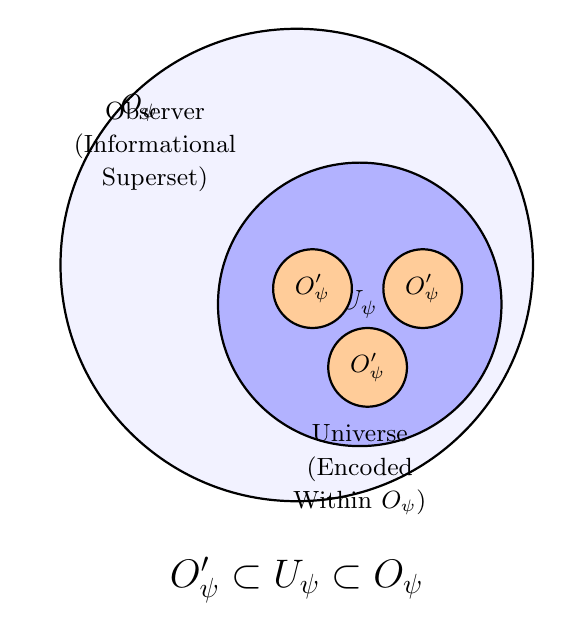
\begin{tikzpicture}
        % Observer O_\psi (Superset)
        \draw[thick, fill=blue!5] (0,0) circle (3cm);
        \node at (-2,2) {\textbf{$O_{\psi}$}};
        \node[text width=3cm, align=center] at (-1.8,1.5)
            {\small Observer\\(Informational Superset)};

        % Universe U_\psi (Encoded Subset)
        \draw[thick, fill=blue!30] (0.8,-0.5) circle (1.8cm);
        \node at (0.8,-0.5) {\textbf{$U_{\psi}$}};
        \node[text width=3cm, align=center] at (0.8,-2.6)
            {\small Universe\\(Encoded Within $O_{\psi}$)};

        % Other Observers O'_\psi
        \draw[thick, fill=orange!40] (0.2,-0.3) circle (0.5cm);
        \node at (0.2,-0.3) {\small \textbf{$O'_{\psi}$}};

        \draw[thick, fill=orange!40] (1.6,-0.3) circle (0.5cm);
        \node at (1.6,-0.3) {\small \textbf{$O'_{\psi}$}};

        \draw[thick, fill=orange!40] (0.9,-1.3) circle (0.5cm);
        \node at (0.9,-1.3) {\small \textbf{$O'_{\psi}$}};

        % Set relation
        \node at (0,-4) {\Large $O'_{\psi} \subset U_{\psi} \subset O_{\psi}$};
    \end{tikzpicture}
    \caption{Wavefunction-indexed encoding: the universe and other observers exist only as structures within the observer’s wavefunction.}
\end{figure}
